\documentclass[a4paper]{article}
\usepackage{fancyhdr}
\usepackage{amsmath}
\usepackage{xcolor}
\usepackage{graphicx}
\usepackage{latexsym}
\usepackage{amssymb}

%% New commands
\newcommand{\eqdef}{\;\stackrel{\text{def}}{=}\;}

\begin{document}
\title{Distributed Systems: Programming Assignment}
\author{David Benamine \& Rodolphe Lepigre\\
        MOSIG - Parallel, Distributed and Embedded Systems}
\date{\today}
\maketitle

%%%%%%%%%%%%%%%%%%%%%%%%%%%%%%%%%%%%%%%%%%%%%%%%%%%%%%%%%%%%%%%%%%%%%%%%%%%%%%
\section*{Introduction}
% TODO

%%%%%%%%%%%%%%%%%%%%%%%%%%%%%%%%%%%%%%%%%%%%%%%%%%%%%%%%%%%%%%%%%%%%%%%%%%%%%%
\section*{Simulator architecture}
% TODO

%%%%%%%%%%%%%%%%%%%%%%%%%%%%%%%%%%%%%%%%%%%%%%%%%%%%%%%%%%%%%%%%%%%%%%%%%%%%%%
\section*{Two regular total-order broadcast protocols}
% TODO

\subsection*{First protocol}
% TODO (good latency)

\subsection*{Second protocol}
% TODO (good throughput with N senders)

%%%%%%%%%%%%%%%%%%%%%%%%%%%%%%%%%%%%%%%%%%%%%%%%%%%%%%%%%%%%%%%%%%%%%%%%%%%%%%
\section*{Theoretical analysis}
% TODO

\subsection*{First protocol}
% TODO
\begin{itemize}
    \item Optimized for latency
    \item Bad throughput
    \item Every broadcast go through the same tree
    \item $P_0$ is always the broadcast initiator
    \item $P_0$ is responsible for the order
    \item if $P_i$ want to send a message, he sent it to 0 who do the broadcast
    \item Latency : log(N) + 1 (send to 0)
    \item Throughput : todo
\end{itemize}
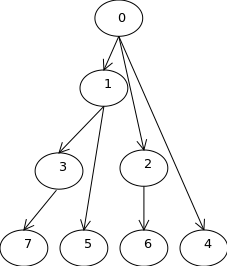
\includegraphics[width=0.5\textwidth]{latencyTO.png}

\subsubsection*{Latency}

\subsubsection*{Throughput}
% TODO

\subsection*{Second protocol}
% TODO
\begin{itemize}
    \item Optimized for throughput
    \item Aller retour
    \item pipeline
    \item retour sur le pipeline inverse
    \item chaque processus reordonne
    \item delivre si 1 ack recu ET en tete de file
    \item voir TO protocol cours Gruber
    \item trois processus debit 4/3
    \item On acquite la tête de file
\end{itemize}
\subsubsection*{Latency}
% TODO

\subsubsection*{Throughput}
% TODO

%%%%%%%%%%%%%%%%%%%%%%%%%%%%%%%%%%%%%%%%%%%%%%%%%%%%%%%%%%%%%%%%%%%%%%%%%%%%%%
\section*{Empirical evaluation}
% TODO

%%%%%%%%%%%%%%%%%%%%%%%%%%%%%%%%%%%%%%%%%%%%%%%%%%%%%%%%%%%%%%%%%%%%%%%%%%%%%%
\section*{Conclusion}
% TODO

\end{document}

